%!TEX root = /Users/markelikalderon/Documents/Git/formwithoutmatter/formwithoutmatter.tex
\chapter{Color} % (fold)
\label{cha:color}

Aristotle defines color as the power to move what is actually transparent (\emph{De Anima} \textsc{ii}.7 418\( ^{a} \)31--418\( ^{b} \)33; \textsc{ii}.7 419\( ^{a} \)10--12).

First, as \citet[367]{Hicks:1907uq} observes, by motion Aristotle does not mean locomotion or change in position. Rather, in \emph{De Anima}, \emph{kinēsis} is Aristotle's general term for change of any kind. Thus \emph{kinētikon} in Aristotle's definition means productive of change rather than productive of spatial movement, more narrowly.

Second, and frustratingly, Aristotle does not directly specify the nature of the change color induces in the transparent medium it acts upon. Indeed, in \emph{De Anima} \textsc{ii}.7 the only effect of color discussed is the effect in terms of which the transparent is defined---the transparent is not visible in itself, but \emph{owning its visibility to the color of another thing}. Is this change, the rendering visible of the transparent, sufficient to understand Aristotle's definition? If it is, this would explain Aristotle's apparent silence about the nature of the change induced in the transparent by color---he merely says nothing \emph{further}, having \emph{already} specified the nature of the change in his definition of the transparent. Given the paucity of textual evidence, a conservative strategy would begin with this hypothesis and only abandon it in favor of speculation should it prove to be an insufficient basis for understanding Aristotle's definition.

Third, a doubt may be registered about the occurrence of transparency in Aristotle's definition. Color is a proper object of sight, and, as such, partly defines the nature of sight. It might reasonably be thought that color could only play a role in defining sight if it had a nature independent of sight. But defining color in terms of the power to move what is actually transparent potentially threatens this order of explanation given the definitional connection between transparency and visibility. It is on these grounds that \citet{Zabarella:1605kx} rejects Aristotle's definition \citep[see][for discussion]{Broackes:1999uq}.

\section{The Generation of the Hues} % (fold)
\label{sec:the_generation_of_the_hues}

The presence of the fiery substance illuminates the potentially transparent me\-di\-um. White (\emph{leukon}) corresponds to this positive determinant of what is actually transparent. Conversely, the absence of the fiery substance darkens the potentially transparent medium. Thus black (\emph{melaton}) corresponds to the absence of this positive determinant of what is actually transparent. White and black are thus associated with a fundamental condition on the visibility of remote external particulars. No doubt in part because of this Aristotle attempts to explain the other hues in terms of the ratio of white and black. He considers three such accounts, in terms of (1) juxtaposition, (2) overlap, and (3) mixture, advocating the third. This can seem surprising. How can the ratio of black and white result in something appearing red? Would it not instead appear gray? Thus \citet[210]{Hett:2000fk} writes that Aristotle's ``doctrine could hardly have survived a few experiments with pigments''. Aristotle's account of the generation of the hues may be surprising, but it would be wrong to prematurely dismiss it. 

The first thing to observe is that \emph{leukon} and \emph{melaton} are better understood as light and dark, rather than white and black. There is a general tendency in Greek color vocabulary to classify colors in terms of relative brightness rather than hue \citep[see][]{Platnauer:1921bh,Lloyd:2007fk}. Traces of such a usage exist in English. Thus we speak of white wine and white people, though neither are white in hue. Similarly neither black people nor black grapes are black in hue. This usage in English, however, does not seem to be perfectly general but is rather lexically determined. It is not the case that for any noun \( N \), the occurrence of ``white'' in \( \ulcorner [white_{Adj}][N_{N}] \urcorner \) can be interpreted in terms of relative brightness instead of hue. The availability of such an interpretation seems to be limited to the adjective's application to certain nouns. The more general usage in Greek is philosophically significant, for it transforms Aristotle's claim. Aristotle is not claiming that the hues are determined by the ratio of white and black, but that they are determined by the ratio of light and dark. And this latter thought is not implausible. As I will argue below, it is an ancient prefiguration of modern reflectance theories \citep[see][]{Hilbert:1987jq}.

Two further considerations are relevant. First, there are a range of observable phenomena that support Aristotle's fundamental claim that ratio of white and black (or light and dark) can give rise to chromatic appearances. Importantly, Aristotle himself provides an example, though in a different context. Second, Aristotle's account has ancient precedent. Thus when Theophrastus discusses Democritus's view that there are four primary colors, he contrasts it with the then dominant view that white and black are the two primary colors:
\begin{quote}
    But first of all, his increase of the number of primaries presents a difficulty; for the other investigators propose white and black as the only simple colours. (\emph{De Sensibus} 79; 68 A 135 DK; \citealt{Stratton:1917vn})
\end{quote}
Arguably, Parmenides and Empedocles are among the ancient thinkers who propose white and black as the only simple colors. Before discussing Aristotle's account of the generation of the hues, then, I will review some empirical support for its central idea, and will discuss the precedent for this doctrine in Parmenides and Empedocles.

In 1894, an English toy maker, Charles Benham, devised a top adorned with a black and white pattern (see Figure~\ref{fig:2}). Sold through Messrs. Newton and Co., an announcement of the ``Artificial Spectrum Top'' was published in \emph{Nature}:
	\begin{quote}
		The top consists of a disc, one half of which is black, while the other half has twelve arcs of concentric circles drawn upon it. Each arc subtends an angle of forty-five degrees. In the first quadrant there are three such concentric arcs, in the next three more, and so on; the only difference being that the arcs are parts of circles of which the radii increase in arithmetical progression. Each quadrant thus contains a group of arcs differing in length from those of the other quadrants. The curious point is that when this disc is revolved, the impression of concentric circles of different colors is produced upon the retina. If the direction of rotation is reversed, the order of these tints is also reversed. \citep{Benham:1894kx}
	\end{quote}
Specifically, if rotated clockwise, the innermost arcs form reddish rings, the next greenish rings, the next light blue rings, and the outermost arcs form violet rings. If rotated counterclockwise, the pattern is reversed with the innermost arcs now forming violet rings and the outermost reddish rings. The apparent colors of Benham's spinning disk are the ``subjective colors'' first described by \citep{Fechner:1838vn} and, hence, are also sometimes described as ``Fechner-Benham colors''.

\begin{figure}[ht]
    \begin{center}
        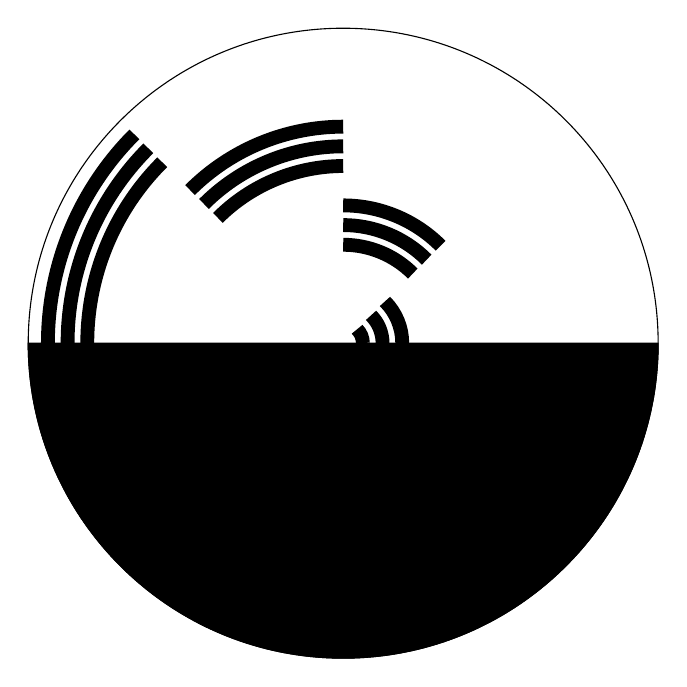
\begin{tikzpicture}
			\draw (0,0) circle (4cm);
			\filldraw[fill=black] (0,0) -- (4cm,0cm) arc (0:-180:4cm) --cycle;
			\draw[line width=5pt] (canvas polar cs:angle=0,radius=0.25cm) arc (0:45:0.25cm);
			\draw[line width=5pt] (canvas polar cs:angle=0,radius=0.50cm) arc (0:45:0.50cm);
			\draw[line width=5pt] (canvas polar cs:angle=0,radius=0.75cm) arc (0:45:0.75cm);
			\draw[line width=5pt] (canvas polar cs:angle=45,radius=1.25cm) arc (45:90:1.25cm);
			\draw[line width=5pt] (canvas polar cs:angle=45,radius=1.50cm) arc (45:90:1.50cm);
			\draw[line width=5pt] (canvas polar cs:angle=45,radius=1.75cm) arc (45:90:1.75cm);
            \draw[line width=5pt] (canvas polar cs:angle=90,radius=2.25cm) arc (90:135:2.25cm);
			\draw[line width=5pt] (canvas polar cs:angle=90,radius=2.50cm) arc (90:135:2.50cm);
			\draw[line width=5pt] (canvas polar cs:angle=90,radius=2.75cm) arc (90:135:2.75cm);
			\draw[line width=5pt] (canvas polar cs:angle=135,radius=3.25cm) arc (135:180:3.25cm);
			\draw[line width=5pt] (canvas polar cs:angle=135,radius=3.50cm) arc (135:180:3.50cm);
			\draw[line width=5pt] (canvas polar cs:angle=135,radius=3.75cm) arc (135:180:3.75cm);
		\end{tikzpicture}
    \end{center}
    \caption{The Benham Disk or ``Artificial Spectrum Top''}
    \label{fig:2}
\end{figure}

Consider a puzzling aspect of the subjective colors of the Benham disk. Each of the spinning arcs reflect light with the same spectral content and with equal average luminance. In advance of observing the spinning disk, one might reasonably expect the spinning arcs to appear as gray rings of equal brightness. Why, then, do the rings appear reddish, greenish, light blue, and violet? The subjective colors of the Benham disk are not completely understood \citep[for a review of some of the color science see][]{Campenhausen:1995yq}. However, this much is clear: The innermost ring appearing reddish is the result of the visual system visually integrating temporal inhomogeneities presented by the spinning disk. Presentations of black and white stimuli altering at a particular temporal ratio elicits a chromatic response in normal human perceivers. 

This basic principle was used in a prototype color television broadcasting system \citep[]{Butterfield:1968uq,Butterfield:1970kx}. Developed by James F. Butterfield, the broadcasting system consists of the Butterfield color encoder that produces a monochromatic signal which when broadcast and displayed on a monitor presents a chromatic appearance. The Butterfield encoder extracts a monochromatic signal from the colored scene by passing the light from the scene through cyan, magenta, and yellow filters. A colored object will appear black when seen through a filter of a complementary color. The filters themselves are arranged in a modified Benham Disk (see Figure~\ref{fig:3}).


\begin{quote}
    When electronic color was first publicly demonstrated in the Los Angeles area over KNXT, no prior announcement had been made at the request of a soft-drink manufacturer sponsoring the test. The beverage firm wanted its color commercials to be a complete surprise to viewers of black-and-white receivers. And, the telecasts were that, to say the very least. Within hours of the electronic-color broadcast, thousands of viewers began asking the same question, ``What happened? Did I really see color on my black-and-white receiver? Or am I having hallucinations?'' \citep[]{Griffin:1968fk}
\end{quote}




\begin{figure}[ht]
    \begin{center}
        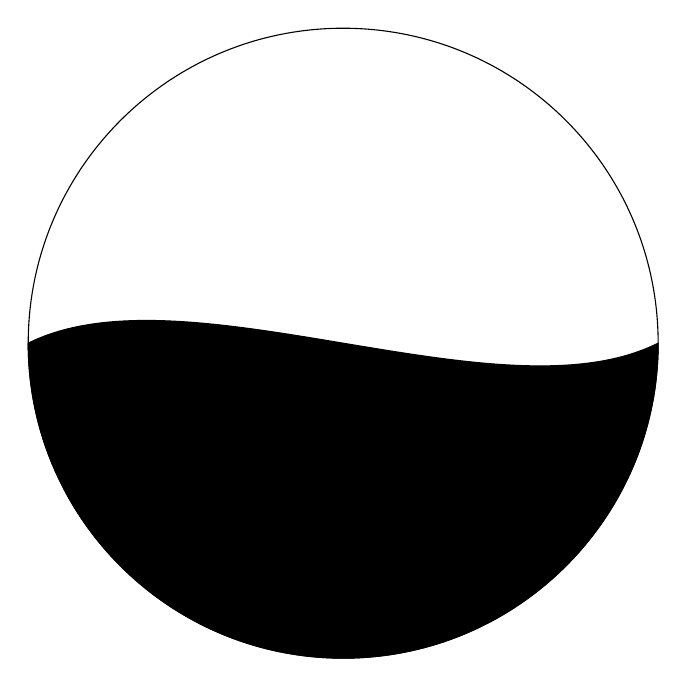
\begin{tikzpicture}
          \draw (0,0) circle (4cm);
          \filldraw (-4cm,0cm) .. controls (-2cm,1cm) and (2cm, -1cm) .. (4cm,0cm) arc (0:-180:4cm) --cycle;;
      \end{tikzpicture}
    \end{center}
    \caption{The filter of the Butterfield Encoder}
    \label{fig:3}
\end{figure}

% section the_generation_of_the_hues (end)

\begin{quote}
    The Apollodorian accomplishment and that artist's importance in the art-historical record as it has come down to us from ancient times can only be explained if he was somehow able to synthesize earlier, less successful attempts, so that a systematic relationship between chiaroscuro and color was established in some consistent manner. Such an accomplishment and nothing les (when we consider the rather late fifth-century dates we must assume for the career of this artist) might have struck the imagination of the ancient viewer as anything so dramatic as an ``invention''. Then Zeuxis, who ``walked through the doors'' that his teacher, Apollodorus, had opened, must have been able to develop more sophisticated variations of the earlier methods. In his own mature work, he must have departed in some striking manner from the system of shading that had characterized his master's pictures; the likelihood is that Zeuxis inveented a kind of chiaroscuro in which the relationship of color to dark and light was definitely altered, in which shading assumed a more dominant role and the nuances of coloring and brushwork became more and more complex, perhaps more ``painterly''. \citep[29]{Bruno:1977fk}
\end{quote}


% chapter color (end)
